\section{Distribuição de média e variância amostrais}
\begin{frame}{Distribuição de média e variância amostrais}
 \begin{itemize}
  \item Distribuição conjunta de $\Sm$ e $\Sv$;
  \item No caso Normal, $\Sm \indep \Sv$ são idependentes!
  \item Distribuição t de Student.
 \end{itemize}
\end{frame}

\begin{frame}{Distribuição de $\Sm$ e $\Sv$}
 \begin{itemize}
  \item $\Sm \sim \operatorname{Normal}\left(\mu, \frac{\sigma^2}{n}\right)$;
  \item $\Sv \sim \operatorname{Gama}\left(\frac{n-1}{2},  \frac{n}{2\sigma^2}\right)$
 \end{itemize}
 \begin{figure}[!ht]
\label{fig:sample_moments_normal}
\begin{center}
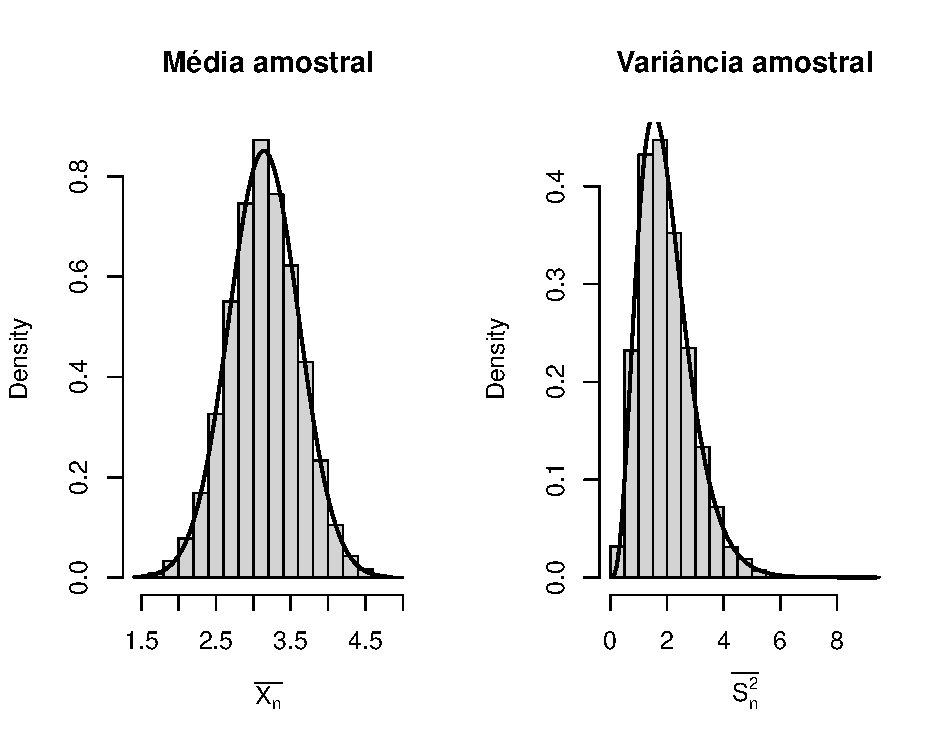
\includegraphics[scale=0.5]{figures/sample_moments_normal.pdf} 
\end{center} 
\end{figure} 
\end{frame}

\begin{frame}{Um Teorema importante}
 Aqui vamos ver um caso especial do Teorema de Basu\footnote{Debabrata Basu (1924--2001) foi um importante estatístico indiano.}, que fala que os dois primeiros momentos amostrais da distribuição Normal são independentes.
 \begin{theo}[Independência da média e variância amostrais na Normal]
 \label{thm:independence_sample_mean_variance_normal}
  Seja $\rs$ uma amostra aleatória de uma distribuição Normal com parâmetros $\mu$ e $\sigma^2$.
  Então a média amostral, $\Sm$ e a variância amostral, $\Sv$, são independentes.
  Ademais, $\Sm \sim \operatorname{Normal}\left(\mu, \frac{\sigma^2}{n}\right)$ e $\Sv \sim \operatorname{Gama}\left(\frac{n-1}{2},  \frac{n}{2\sigma^2}\right)$.
 \end{theo}
\textbf{Prova:} Troca de variáveis em duas dimensões; propriedades de matrizes ortogonais.
Ver Teorema 8.3.1 em DeGroot (prova na pág. 476).
\end{frame}

\begin{frame}{Exemplo}
 Suponha que queremos determinar o tamanho de amostra, $n$, de modo que os EMVs da média $\mu$ e do desvio padrão $\sigma$ estejam ``perto'' dos seus valores verdadeiros.
 Formalmente, queremos encontrar $n$ tal que
 \[ \pr\left( \left|\hat{\mu} - \mu\right| \leq \frac{1}{5}\sigma \: \text{\underline{e}} \: \left|\hat{\sigma}-\sigma\right| \leq  \frac{1}{5}\sigma \right) \geq \frac{1}{2} ,\]
 seja satisfeito.
\end{frame}

\begin{frame}{A distribuição $t$ de Student}
 Qual a distribuição de $\frac{\sqrt{n}\left(\Sm - \mu\right)}{\hat{\sigma}}$?
 A resposta é a distribuição t de ``Student''\footnote{William Sealy Gosset (1876--1937) foi um estatístico inglês que, em 1908, publicou o resultado acima sob o pseudônimo ``Student'', ou estudante/aluno.}
 
 \begin{defn}[A distribuição t]
 \label{def:Student_t_distribution}
  Considere duas variáveis aleatórias, $Y \sim\operatorname{Qui-quadrado}(m)$ e $Z \sim\operatorname{Normal}(0, 1)$ e defina a variável aleatória
  \[ X = \frac{Z}{\sqrt{\frac{Y}{m}}}. \]
 Dizemos que $X$  tem distribuição~\textbf{t de Student com $m$ graus de liberdade}. 
 Sabemos ainda que
 \[f_X(x) = \frac{\Gamma(\frac{m + 1}{2})}{\sqrt{m\pi}\Gamma(\frac{m}{2})} \left(1 + \frac{x^2}{m}\right)^{-\frac{m+1}{2}},\: x \in (-\infty, \infty). \]
 \end{defn}
Para $m>2$, $E[X] = 0$ (porquê?) e $\vr(X) = m/(m-2)$.
\end{frame}

\begin{frame}{Comparando a t com outras distribuições}
\begin{figure}[!ht]
 \begin{center}
  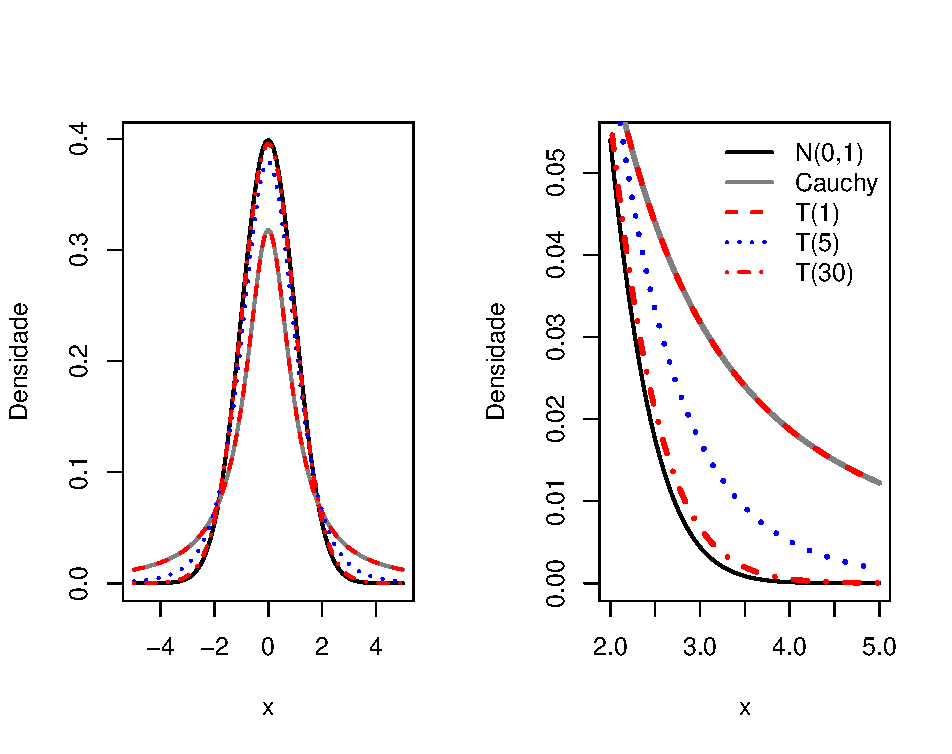
\includegraphics[scale=.6]{figures/comparacao_t_Student.pdf}
 \end{center}
\end{figure} 
\end{frame}

\begin{frame}{Um exemplo}
\begin{theo}[Distribuição amostral do estimador não-viesado da variância]
\label{thm:unbiased_variance_estimator_StudentT}
 Considere o estimador 
 \begin{equation*}
  \hat{\sigma}^\prime = \sqrt{\frac{\Delta^2}{n-1}},
 \end{equation*}
onde $\Delta^2 = \sum_{i=1}^n \left(X_i - \Sm\right)^2$.
Então 
\begin{equation*}
 \frac{\sqrt{n}\left(\Sm - \mu\right)}{\hat{\sigma}^\prime} \sim \operatorname{Student}(n-1).
\end{equation*}
\end{theo}
\textbf{Prova:}
Ver Teorema 8.4.2 em DeGroot.
Defina $Z = \sqrt{n}(\Sm - \mu)/\sigma$ e $Y = \Delta^2/\sigma^2$.
Então $Z \sim\operatorname{Normal}(0,1)$ e $Y\sim\operatorname{Qui-quadrado}(n-1)$.
Faça
\begin{equation}
 U = \frac{Z}{\sqrt{\frac{Y}{n-1}}} = \frac{\sqrt{n}(\Sm-\mu)}{\sqrt{\frac{\Delta^2}{n-1}}},
\end{equation}
e note que $U \sim \operatorname{T}(n-1)$  $\qed$
\end{frame}

\begin{frame}{O que aprendemos?}
\begin{itemize}

  \item[\faLightbulbO] Independência dos momentos amostrais da Normal;    
  
   ``Numa amostra aleatória Normal, $\Sm$ e $\Sv$ são independentes e $\Sm \sim \operatorname{Normal}\left(\mu, \frac{\sigma^2}{n}\right)$ e $\Sv \sim \operatorname{Gama}\left(\frac{n-1}{2},  \frac{n}{2\sigma^2}\right)$.''  
     
   \item[\faLightbulbO] A distribuição t de Student;
   
   ``A diferença padronizada entre a média amostral e a média populacional ($\mu$) tem distribuição t de Student, que não depende de $\sigma^2$''
    
  \end{itemize}
 \end{frame}

\begin{frame}{Leitura recomendada}
\begin{itemize}
 \item[\faBook] DeGroot seções 8.3 e 8.4;
%  \item[\faBook] $^\ast$ Casella \& Berger (2002), seção 6.2.
%  \item[\faBook] $^\ast$ Schervish (1995), capítulo 7.
 \item[\faForward] Próxima aula: DeGroot, seção 8.5;
 \item {\large\textbf{Exercícios recomendados}}
 \begin{itemize}
  \item[\faBookmark] DeGroot.
  \begin{itemize}
   \item Seção 8.3: exercício 8;
   \item Seção 8.4: derivar a densidade da Distribuição t de Student.
  \end{itemize}   
  \end{itemize}
 \end{itemize} 
\end{frame}
